% debut d'un fichier latex standard
\documentclass[a4paper,12pt,oneside]{article}
\usepackage[top=3cm, bottom=3.5cm]{geometry}
% pour l'inclusion de figures en eps,pdf,jpg,....
\usepackage{graphicx}
\usepackage{wrapfig}
% quelques symboles mathematiques en plus
\usepackage{amsmath}
% le tout en langue francaise
\usepackage[french]{babel}
% on peut ecrire directement les characteres avec l'accent
% a utiliser sur Linux/Windows
\usepackage[utf8]{inputenc}
% a utiliser sur le Mac
%\usepackage[applemac]{inputenc}
% pour l'inclusion de links dans le document (pdflatex)
\usepackage[colorlinks,bookmarks=false,linkcolor=blue,urlcolor=blue]{hyperref}
%
\usepackage{caption}
\usepackage{float}
% quelques abreviations utiles
\def \be {\begin{equation}}
\def \ee {\end{equation}}
\def \dd  {{\rm d}}
\newcommand{\norme}[1]{\left\Vert #1 \right\Vert}
%
\newcommand{\mail}[1]{{\href{mailto:#1}{#1}}}
\newcommand{\ftplink}[1]{{\href{ftp://#1}{#1}}}
%
%%%%%%%%%%%%%%%%%%%%%%%%%%%%%%%%%% le document commence ici %%%%%%%%%%%%%%%%%%%%%%%%%%%%%%%%%%%%%%%%%%%%
\begin{document}
% le titre et l'auteur
\title{Physique numérique I : exercice 2}
\date{\today}
\author{Victor Despland, Timothée Dao\\{\small \mail{victor.despland@epfl.ch}, \mail{timothee.dao@epfl.ch}}}
\maketitle
\tableofcontents


%%%%%%%%%%%%%%%%%%%%%%%%%%%%%%%%%%%%%%%%%%%%%%%%%%%%%%%%%%%%%%%%%%%%%%%%%%%%%%%%%%%%%%%%%%%%%%%%%%%%%%%%
\newpage
\section{Introduction}

\intextsep=0cm
\begin{wrapfigure}{r}{0.5\textwidth}
    \centering
    \includegraphics[width=0.3\textwidth]{schemaDonnee}
    \caption{\cite{donneeEX2}}
\end{wrapfigure}


Un proton de masse $m = 1.6726  \times 10^{-27 } \rm kg$, de charge $q = 1.6022 \times 10^{-19} \rm C$, avec une position initiale $\textbf{r}_0 = (x_0, y_0 )$ et une vitesse initiale $\textbf{v}_0 = (v_{x0} , v_{y0} )$, est plongé dans un champ électrique uniforme $\textbf{E} = E\hat{y}$ et un champ magnétique uniforme $\textbf{B} = B\hat{z} $. Il est alors soumis à la force de Lorentz : 
\be
\textbf{F} = q(\textbf{E} + \textbf{v} \times\textbf{ B})
\ee

\intextsep=0.5cm
%%%%%%%%%%%%%%%%%%%%%%%%%%%%%%%%%%%%%%%%%%%%%%%%%%%%%%%%%%%%%%%%%%%%%%%%%%%%%%%%%%%%%%%%%%%%%%%%%%%%%%%
\section{Calculs analytiques}
De la 2ème loi de Newton, $\textbf{F}=m\Dot{\textbf{v}}$, et de $\textbf{v}=\Dot{\textbf{r}}$ on tire le système d'équations différentielles caractérisant notre problème :
\be
\frac{\dd }{\dd t} 
\left( \begin{array}{c} v_x \\ v_y \\ x \\ y \end{array} \right)
=
\left( \begin{array}{c}
   \frac{q}{m} v_y B\\ \frac{q}{m} (E-v_x B) \\ 
   v_x \\ v_y
\end{array} \right)
\label{eq1}
\ee
\subsection{Résolution du système dans le cas $E=0$ et $B=B_0$}
Les deux premières équations du système sont autonomes, on commence donc par les résoudre. Dans le cas où $E=0$ et $B=B_0$, ça se résume à résoudre :
\be
\frac{\dd }{\dd t} 
\left( \begin{array}{c} v_x \\ v_y \end{array} \right)
=
\Omega
\left( \begin{matrix}
 0 & 1 \\
 -1 & 0
\end{matrix} \right)
\left( \begin{array}{c}
   v_{x_0} \\ v_{y_0}
\end{array} \right), \quad
\textbf{v}(0) = \textbf{v}_0
\ee
avec $\Omega=\frac{qB_0}{m}$.
La solution est donnée par \footnote{c.f. référence \cite{stubbe}} 
\be
\textbf{v}(t)=\exp\left( \begin{matrix}
 0 & \Omega t \\
 -\Omega t & 0
\end{matrix} \right) 
\left( \begin{array}{c}
   v_{x_0} \\ v_{y_0}
\end{array} \right)
=
\left( \begin{array}{c}
   v_{x_0}  \cos (\Omega t) + v_{y_0} \sin (\Omega t) \\
   -v_{x_0} \sin (\Omega t) + v_{y_0} \cos (\Omega t)
\end{array} \right)
\ee
On résout finalemement les deux dernières équations du système :
\be
\frac{\dd }{\dd t} 
\left( \begin{array}{c} x \\ y \end{array} \right)
=
\left( \begin{array}{c} v_x \\ v_y \end{array} \right) , \quad
\textbf{r}(0)=\textbf{r}_0
\ee
La solution est donnée par 
\be \label{equaMvmt}
\left( \begin{array}{c} x \\ y \end{array} \right) (t)
=
\frac{1}{\Omega} \left( \begin{array}{c}
   v_{x_0}  \sin (\Omega t) - v_{y_0} \cos (\Omega t) + v_{y_0} + \Omega x_0 \\
   v_{x_0} \cos (\Omega t) + v_{y_0} \sin (\Omega t) - v_{x_0} + \Omega y_0
\end{array} \right) 
\ee
\subsection{Position initiale}
Étant donné $v_{x_0}=0$ et $v_{y_0}=v_0$, on cherche la position initiale $\textbf{r}_0$ telle que la trajectoire soit centrée en  
$(0,0)$. En substituant ces valeurs dans l'équation (\ref{equaMvmt}) on obtient :
\be
\left\{\begin{array}{c}
x(t)-\frac{v_0}{\Omega} -x_0 = -\frac{v_0}{\Omega}\cos (\Omega t)\\
y(t)-y_0 = \frac{v_0}{\Omega}\sin (\Omega t)\\
\end{array} \right.
\ee
En mettant au carré les deux équations et en les additionnant, on obtient l'équation d'un cercle :
\be \label{equaCercle}
(x(t)-\frac{v_0}{\Omega} -x_0)^{2} + (y(t)-y_0)^2 = \frac{v_0^2}{\Omega^2}
\ee
Pour que le cercle soit centré sur l'origine, on doit alors prendre 
\be \label{PosIni}
(x_0,y_0) = (\frac{v_0}{\Omega},0) 
\ee

\subsection{Temps final \label{tFin}}
Étant donnné $v_{x_0}=0$, $v_{y_0}=4\times 10^{5}  \rm m/s$ et $B=3 \rm T$, on calcule la position initiale : $x_0=\frac{v_0}{\Omega}=-1.39\times10^{-5} \rm m$ et $y_{0}=0$. On prend comme instant final $t_{fin}$ tel que le proton effectue théoriquement 5 périodes de rotation : 
\be
T=\frac{2\pi}{\Omega}=\frac{2\pi m}{qB_0}=2.2\times 10^{-8} {\rm s} \quad ;\quad  t_{fin}=5T=1.09 \times 10^{-7} \rm s 
\ee

\subsection{Énergie} 
Dans le cas d'une particule soumis à un champ électrique et magnétique, l'énergie mécanique est conservée. La force électrostatique est conservative  et la force de Lorentz quant à elle n'entre pas en compte dans l'expression de l'énergie mécanique, car son travail est nul. Son expression est donc de la forme :
\be
E_{mec}=E_{pot}+E_{cin}=-qEy+\frac{1}{2}m\|\vec{v}\|^2
\ee
L'énergie potentielle électrostatique est négative car la force électrostatique va dans le même sens que l'axe y. Donc la particule effectuera un travail pour se déplacer dans le sens inverse à l'axe y, le potentiel est donc plus grand sur une position inférieure.

%%%%%%%%%%%%%%%%%%%%%%%%%%%%%%%%%%%%%%%%%%%%%%%%%%%%%%%%%%%%%%%%%%%%%%%%%%%%%%%%%%%%%%%%%%%%%%%%%%%%%%%%
\newpage
\section{Méthodes numériques}
Le système d'équations différentielles définissant ce problème est
\be \label{sysDef}
\textbf{y} =  \left( \begin{array}{c} v_x \\ v_y \\ x \\ y \end{array} \right) , \quad \textbf{f}(\textbf{y},t)=\frac{d\textbf{y}}{dt}= \frac{\dd }{\dd t}\left( \begin{array}{c} v_x \\ v_y \\ x \\ y \end{array} \right) = \left( \begin{array}{c} a_x \\ a_y \\ v_x \\ v_y \end{array} \right)
\ee
Les valeurs de $a_x$ et $a_y$ sont explicitées dans l'équation \eqref{eq1}.

\subsection{Schéma d'Euler \cite{notesDeCours}}
Pour un pas d'itération $\Delta t$, le schéma d'euler explicite  s'obtient en écrivant le développement limité d'ordre 2 pour $y(t_{i+1})$, avec $t_{i+1} = t_{i} + \Delta t$
\be
y(t_{i+1})=y(t_{i})+ \frac{\dd y}{\dd t}(t_i)\Delta t+O(\Delta t^2)
\ee
En négligeant les termes en $O(\Delta t^2)$, en écrivant $y^{i}$ l'approximation de $y(t_{i})$ et utilisant l'eq.\ref{sysDef}, on obtient l'équation du schéma d'Euler:
\be 
\textbf{y}^{i+1}=\textbf{y}^{i}+\textbf{f}(\textbf{y}^i,t_i)\Delta t
\ee
En substituant les valeurs du système d'équation différentielles on obtient:
\be
\left( \begin{array}{c} v_x^{i+1} \\ v_y^{i+1} \\ x^{i+1} \\ y^{i+1} \end{array} \right) =\left( \begin{array}{c} v_x^{i} \\ v_y^{i} \\ x^{i} \\ y^{i} \end{array} \right)
+ \left( \begin{array}{c}
   \frac{q}{m} v_y^{i} B\\ \frac{q}{m} (E-v_x^{i} B) \\ 
   v_x^{i} \\ v_y^{i}
\end{array} \right)\Delta t
\ee
La méthode converge linéairement.

\subsection{Schéma d'Euler-Cromer \cite{notesDeCours}}
La méthode d'Euler-Cromer est similaire à celle d'Euler, on utilise seulement les approximations au temps $t_{i+1}$ dans la fonction $\textbf{f}$ dès qu'on le peut :
\be
\left( \begin{array}{c} v_x^{i+1} \\ v_y^{i+1} \\ x^{i+1} \\ y^{i+1} \end{array} \right) =\left( \begin{array}{c} v_x^{i} \\ v_y^{i} \\ x^{i} \\ y^{i} \end{array} \right)
+ \left( \begin{array}{c}
   \frac{q}{m} v_y^{i} B\\ \frac{q}{m} (E-v_x^{i+1} B) \\ 
   v_x^{i+1} \\ v_y^{i+1}
\end{array} \right) \Delta t
\ee
La convergence est également linéaire.
\label{paraEulerC}
\subsection{Schéma de Runge-Kutta 2 (RK2) \cite{notesDeCours}}
 La méthode RK2 consiste à évaluer d'abord la valeur de la fonction en $t_{i+\frac{1}{2}}$, afin de l'utiliser pour avancer d'un pas de temps complet, c'est-à-dire de $t_i$ à $t_{i+1}$. Pour réaliser cet algorithme, il nous faut alors d'abord calculer deux variables intermédiares, qui sont données par:
\be
\textbf{k}_1=\Delta t\textbf{f}(\textbf{y}_i,t_i)\label{k1}
\ee
\be
\textbf{k}_2=\Delta t\textbf{f}(\textbf{y}_i+\frac{1}{2}\textbf{k}_1,t_{i+
\frac{1}{2}})\label{k2}
\ee
avec $t_{i+\frac{1}{2}}=t + \frac{\Delta t}{2},i=1,2,3,...$ \\
L'approximation de $\textbf{y}^{i+1}$ s'exprime alors par:
\be
\textbf{y}^{i+1}= \textbf{y}^{i}+\textbf{k}_2
\ee
 En remplaçant par les fonctions en \eqref{eq1}, les variables intermédiaires \eqref{k1} et \eqref{k2}  sont données par:
\be
\textbf{k}_1=\Delta t \left( \begin{array}{c}
   \frac{q}{m} v_y^{i} B\\ \frac{q}{m} (E-v_x^{i} B) \\ 
   v_x^{i} \\ v_y^{i}
\end{array} \right)
\ee
\be
\textbf{k}_2=\Delta t  \left( \begin{array}{c}
   \frac{q}{m}B v_y^{i}(1+\frac{qB\Delta t}{2m}) \\ \frac{q}{m} (E-v_x^{i} B)(1-\frac{qB\Delta t}{2m}) \\ 
   v_x^{i}(1+\frac{\Delta t}{2}) \\ v_y^{i}(1+\frac{\Delta t}{2})
\end{array} \right)\label{kk2}
\ee
note: \textit{on obtient  uniquement les valeurs de \eqref{kk2} dans le cas où B et E sont constant.}\\
Cette méthode converge à l'ordre 2.

\subsection{Schéma de Verlet \cite{notesDeCours}}
La méthode de Verlet s'obtient en combinant les deux différentes méthodes d'Euler-Cromer A et B (celle décrite dans le paragraphe \ref{paraEulerC} est la A), chacune pour un demi pas de temps $\Delta t /2$. Ceci nous donne :

\be
\left( \begin{array}{c} v_x^{i+1/2} \\ v_y^{i+1/2} \\ x^{i+1/2} \\ y^{i+1/2} \end{array} \right) 
=
\left( \begin{array}{c} v_x^{i} \\ v_y^{i} \\ x^{i} \\ y^{i} \end{array} \right)
+ 
\left( \begin{array}{c} \frac{q}{m} v_y^{i} B \\ \frac{q}{m} (E-v_x^{i+1/2} B) \\ v_x^{i+1/2} \\ v_y^{i+1/2} \end{array} \right) \frac{\Delta t}{2}
\ee

\be
\left( \begin{array}{c} y^{i+1} \\ x^{i+1} \\ v_y^{i+1} \\ v_x^{i+1} \end{array} \right) 
=
\left( \begin{array}{c} y^{i+1/2} \\ x^{i+1/2} \\ v_y^{i+1/2} \\ v_x^{i+1/2} \end{array} \right)
+
\left( \begin{array}{c} v_y^{i+1/2} \\ v_x^{i+1/2} \\ \frac{q}{m} (E-v_x^{i+1/2} B) \\ \frac{q}{m} v_y^{i+1} B \end{array} \right) \frac{\Delta t}{2}
\ee


%%%%%%%%%%%%%%%%%%%%%%%%%%%%%%%%%%%%%%%%%%%%%%%%%%%%%%%%%%%%%%%%%%%%%%%%%%%%%%%%%%%%%%%%%%%%%%%%%%%%
\newpage
\section{Résultats numériques}
\subsection{Simulations avec $E=0$ et $B=B_0$}
Cette première série de simulations consiste à étudier le cas où la trajectoire est centrée à l'origine, avec un champ électrique nul et un champ magnétique constant. On reprend les mêmes conditions que décrites dans la section \ref{tFin}.
\subsubsection{Étude de convergence}
On réalise une série de simulations pour les quatre schémas, en faisant varier le nombre de pas de temps $N_{steps}$ entre $10^2$ et $10^5$. Pour chaque simulation, le pas de temps vaut $\Delta t = t_{fin}/N_{steps}$. On compare ensuite les valeurs données par les simulations numériques, $\textbf{r}_i=(x_i,y_i)$, et par la solution analytique $\textbf{r}(t_i)=(x(t_i),y(t_i))$, avec $t_i=i \times \Delta t$ et $i=0,...,N_{steps}$. Pour chaque simulation, on retient le maximum de l'erreur sur la position $e=\max_{i=0,...,N_{steps}} \norme{\textbf{r} (t_i) - \textbf{r}_i}$.

\begin{figure}[h]
\centerline{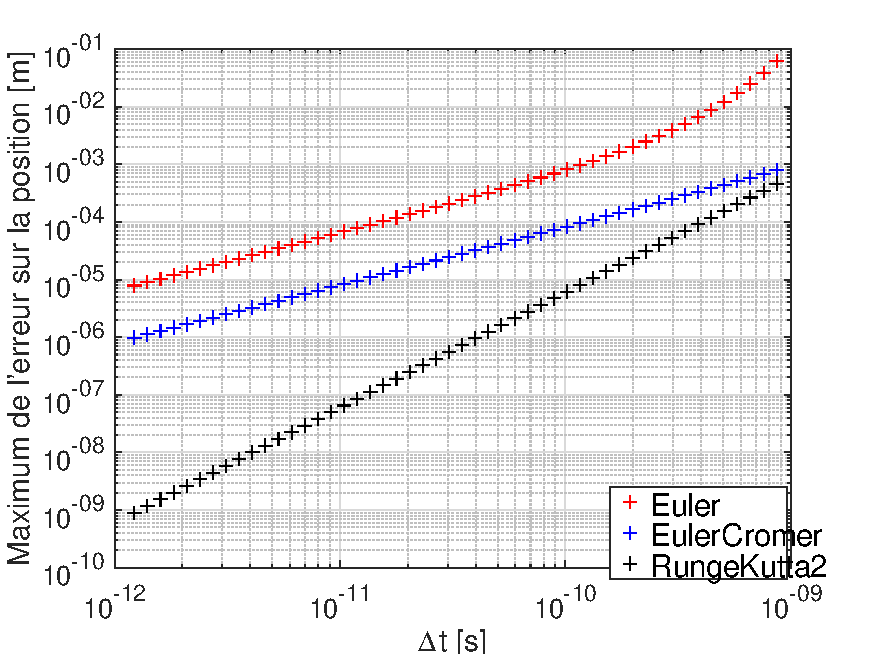
\includegraphics[width=0.95\linewidth,angle=0]{etudeSchema/etudeConv}}
\caption{ \label{etudeConv}\em
 Maximum de l'erreur sur la position (m) en fonction du pas de temps $\Delta t$ (s) sur une échelle log-log pour les schémas d'Euler, d'Euler-Cromer, de Runge-Kutta 2 et de Verlet.
}
\end{figure}

Les résulats sont présentés sur la Fig.\ref{etudeConv} et on peut donc confirmer l'ordre des méthodes qui est de : 
\begin{itemize}
    \item 2 pour RK2 et Verlet
    \item 1 pour Euler et Euler-Cromer
\end{itemize} 
en constatant que leurs pentes sont égales à deux et respectivement un. On constate cependant une courbure sur le graphe d'Euler quand $\Delta t >10^{-10}$, ceci étant du a l'instabilité du schéma, traitée à la section \ref{stabilite}.


\subsubsection{Étude de stabilité \label{stabilite}}
\paragraph{Orbites}
On présente ici les orbites réalisée numériquement avec plusieurs pas de temps $\Delta t$. La trajectoire théorique a également été ajoutée aux graphes.

Pour la méthode d'Euler (Fig.\ref{etudeStabiliteXYEuler}), les trajectoires forment des spirales et finissent par "exploser", ce qui est la signature d'une instabilité numérique.

Pour la méthode d'Euler-Cromer (Fig.\ref{etudeStabiliteXYEulerCromer}), les trajectoires numériques sont légèrement décalées par rapport à la théorique, cependant on peut remarquer qu'en augmentant de nombre de pas de temps, on se rapproche de cette dernière et de plus l'aire déterminée par la trajectoire semble conservée peut importe de le nombre de pas de temps.

Quant à la méthode de Runge-Kutta 2 (Fig.\ref{etudeStabiliteXYRungeKutta2}), les trajectoires numériques et théorique se confondent à l'échelle étudiée.

\begin{figure}[H]
\centerline{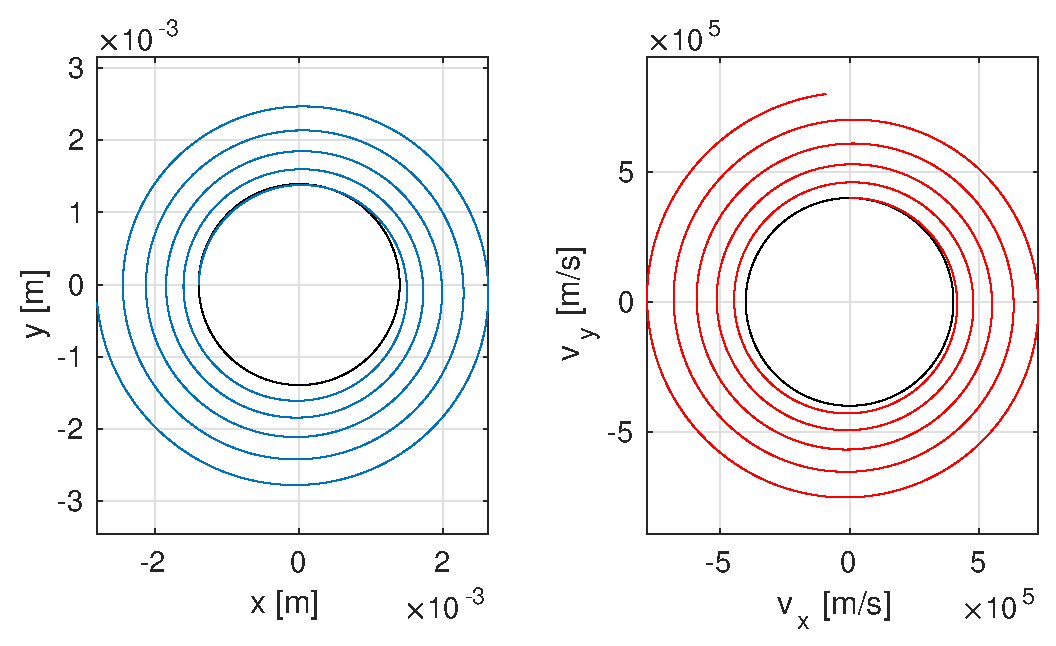
\includegraphics[width=0.95\linewidth,angle=0]{etudeSchema/etudeStabiliteXYEuler}}
    \caption{ \label{etudeStabiliteXYEuler}\em
     Trajectoires (position à gauche et vitesse à droite) d'un proton dans un champ magnétique uniforme et en absence de champ électrique, simulations réalisées avec la méthode d'Euler avec $N_{steps}=700$. Trajectoires théoriques en noir.}
\end{figure}

\begin{figure}[H]
   \centerline{
    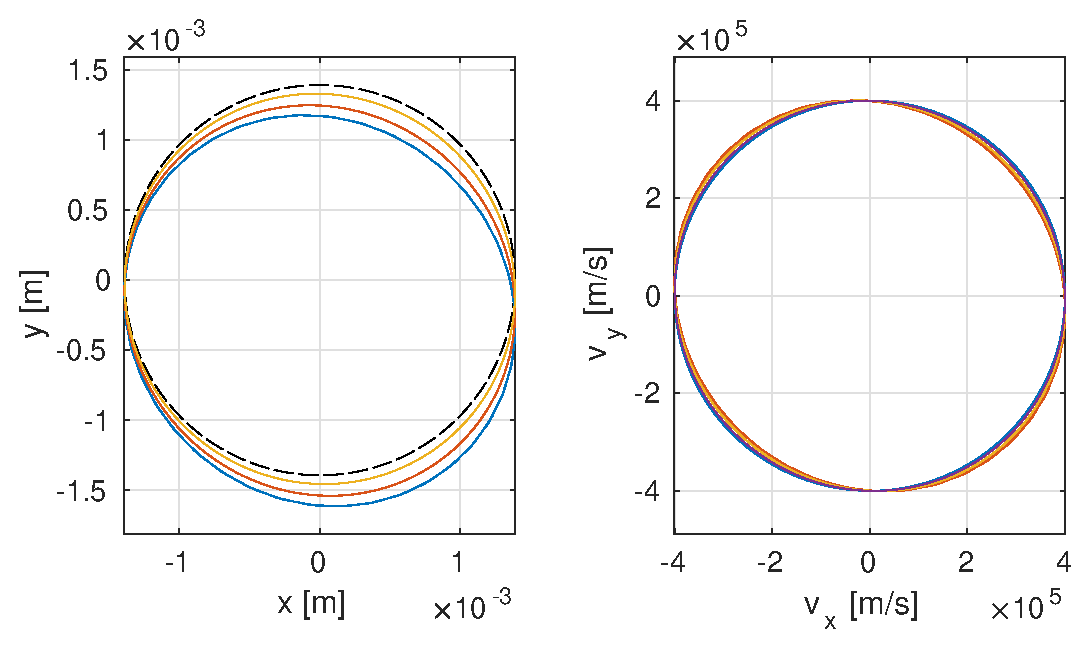
\includegraphics[width=0.95\linewidth,angle=0]{etudeSchema/etudeStabiliteXYEulerCromer}}
    \caption{ \label{etudeStabiliteXYEulerCromer}\em
 Trajectoires (position à gauche et vitesse à droite) d'un proton dans un champ magnétique uniforme et en absence de champ électrique, simulations réalisées avec la méthode d'Euler-Cromer avec $N_{steps}=$ 200 (bleu), 300 (rouge), 700 (jaune). Trajectoires théoriques en noir.}
\end{figure}

\begin{figure}[H]
    \centerline{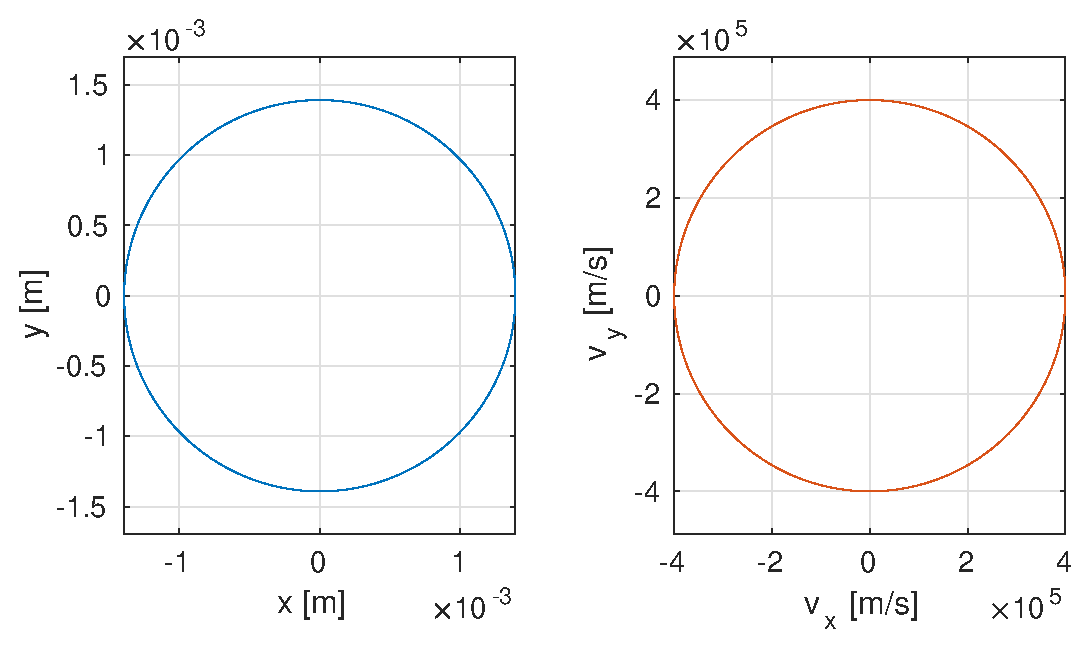
\includegraphics[width=0.95\linewidth,angle=0]{etudeSchema/etudeStabiliteXYRungeKutta2}}
\caption{ \label{etudeStabiliteXYRungeKutta2}\em
Trajectoires (position à gauche et vitesse à droite) d'un proton dans un champ magnétique uniforme et en absence de champ électrique, simulations réalisées avec la méthode de Runge-Kutta avec $N_{steps}=$ 200 (bleu), 300 (rouge), 700 (jaune). Trajectoires théoriques en noir.
}
\end{figure}




\paragraph{Stabilité Euler}
Pour analyser la stabilité de la méthode, on trace un graphe de la position sur $x$ par rapport au temps ainsi que l'évolution temporelle de l'energie mécanique. Comme on est toujours dans le contexte d'un champ électrique nulle, l'expression de l'énergie mécanique se réduit à l'énergie cinétique.
\begin{figure}[H]
\centerline{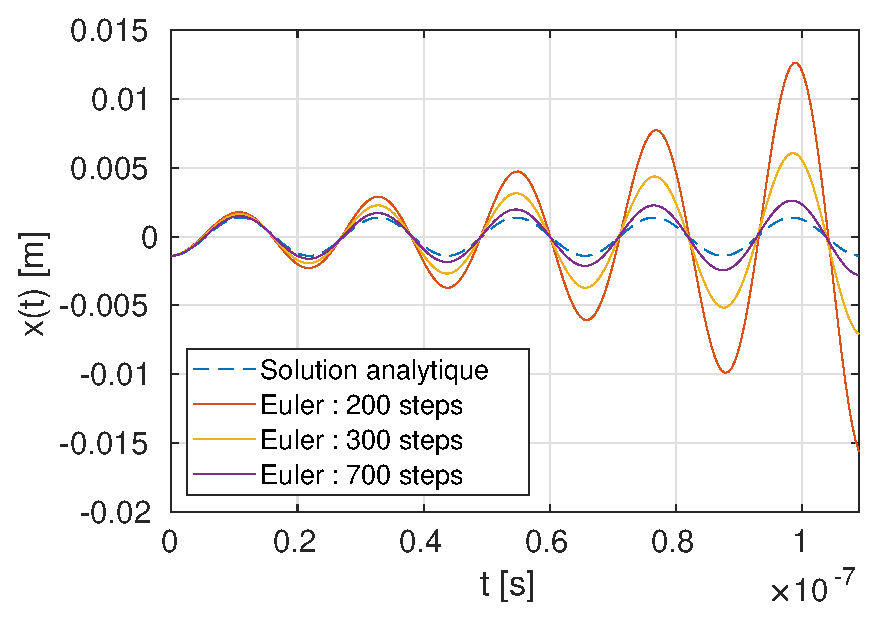
\includegraphics[scale=0.9,angle=0]{etudeSchema/etudeStabilitePosEuler}}
\caption{ \label{etudeStabilitePosEuler}\em
 Position sur x de la particule par rapport au temps avec la méthode d'Euler, en l'absence de champs électrique ($B=B_0$, $E=0$).
}
\end{figure}
\begin{figure}[H]

\centerline{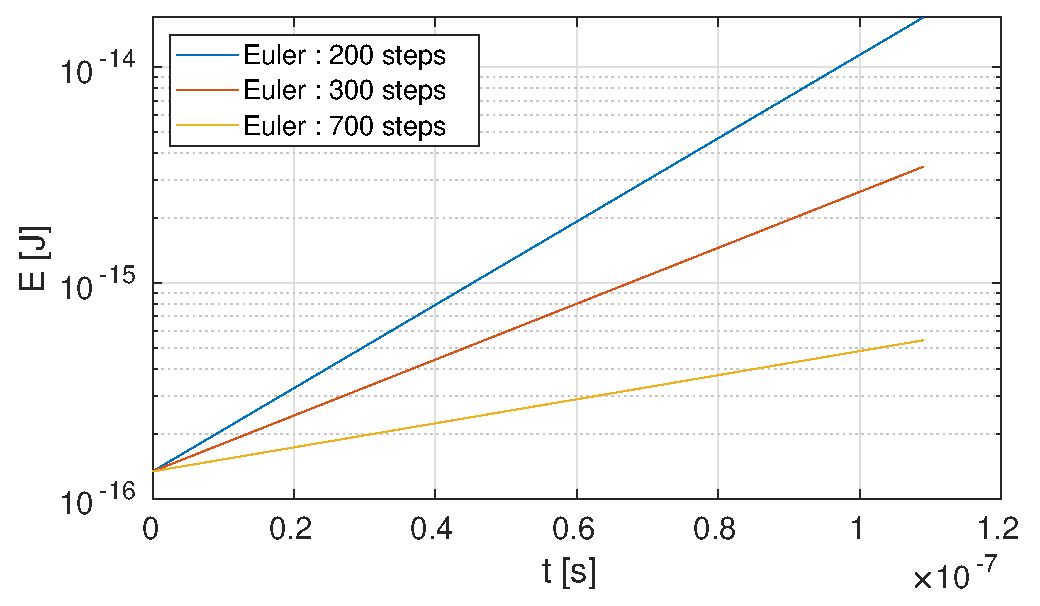
\includegraphics[scale=0.8,angle=0]{etudeSchema/etudeStabiliteEnergyEuler}}
\caption{ \label{etudeStabiliteEnergyEuler}\em
Énergie mécanique de la particule par rapport au temps ($B=B_0$, $E=0$). Simluations réalisées avec la méthode d'Euler.
}
\end{figure}
On peut constater sur la Fig.\ref{etudeStabilitePosEuler} que l'amplitude augmente par rapport au temps, et donc l'erreur aussi. Effectivement, lorsqu'elle est appliquée sur des mouvements de type harmonique, la méthode d'Euler est touours instable. Son amplitude augmente exponoentiellement par rapport à $\Delta t$. L'énergie mécanique augmente également au fil du temps, alors qu'elle devrait être conservée. Cette méthode n'est donc pas conservative.

\paragraph{Stabilité Euler-Cromer}
 On peut constater sur la  Fig.\ref{etudeStabilitePosEulerCromer} que le mouvement simulé par ce schéma avec 3 différentes valeurs de $N_{steps}$ se confondent avec la solution analytique. L'energie quant à elle (Fig.\ref{etudeStabiliteEnergyEulerCromer}), n'est localement pas conservée, si l'on considère l'évolution de l'ordre d'une période. Il est n'est donc pas d'une constance exacte. Cependant, on peut constater que le graphe est périodique et sinusoïdale, de période $T\simeq\frac{1}{2}T_{particule}$. De plus, l'énergie mécanique est conservée en moyenne. Ce schéma est donc stable pour un mouvement harmonique. Le schéma d'Euler-Cromer apporte de nettes améliorations par rapport au schéma d'Euler, pour la position et pour l'énergie, car elle assure une certaine stabilité.
\begin{figure}[H]
\centerline{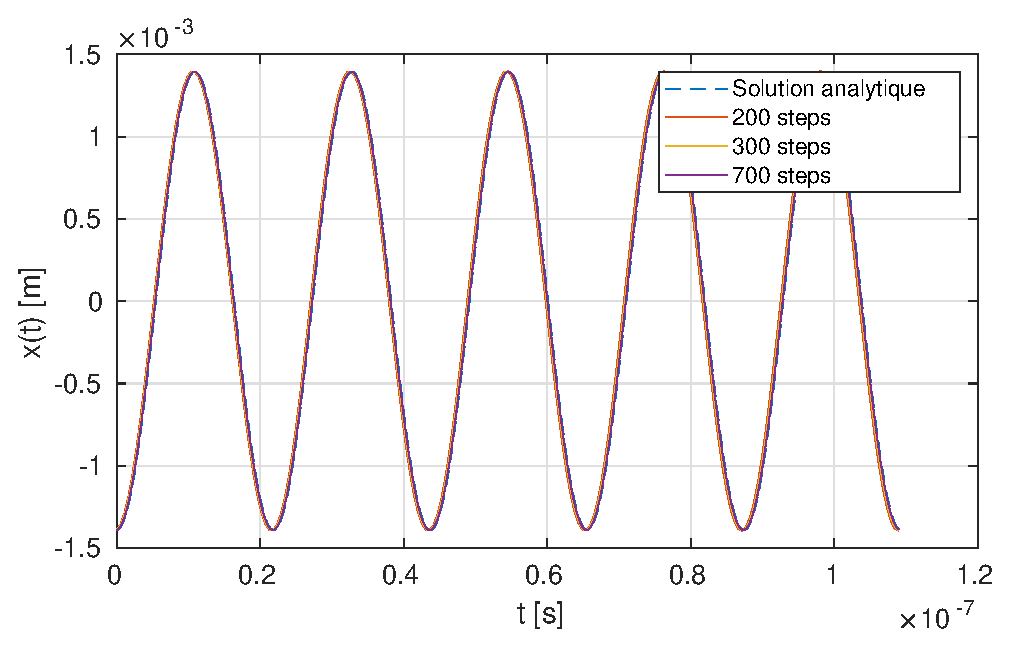
\includegraphics[scale=0.8,angle=0]{etudeSchema/etudeStabilitePosEulerCromer}}
\caption{ \label{etudeStabilitePosEulerCromer}\em
 Position sur x en fonction du temps pour le schéma d'Euler-Cromer avec $E=0$ et $B=B_0$.
}
\end{figure}
\begin{figure} [H]
\centerline{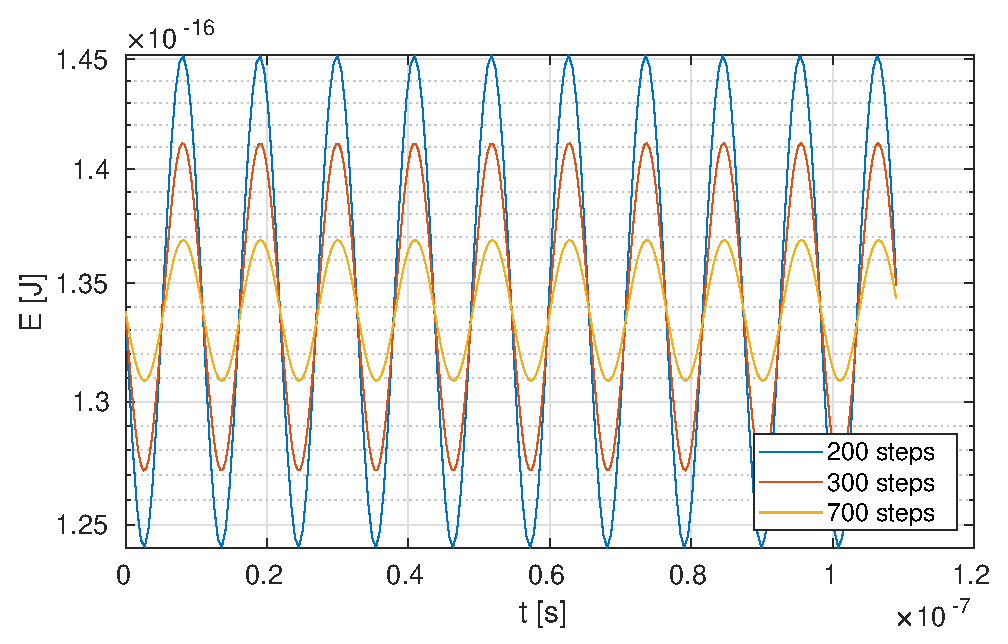
\includegraphics[scale=0.73,angle=0]{etudeSchema/etudeStabiliteEnergyEulerCromer}}
\caption{ \label{etudeStabiliteEnergyEulerCromer}\em
 Énergie mécanique d'un proton en fonction du temps pour le schéma d'Euler-Cromer, avec 3 pas de temps différents ($E=0$ et $B=B_0$).
}
\end{figure}

\paragraph{Stabilité Runge-Kutta}
On constate sur la Fig.\ref{etudeStabiliteEnergyRungeKutta2} que les trajectoires simulées avec RK2 se confondent avec la position issu de la solution analytique. Cependant, l'énergie (Fig.\ref{etudeStabiliteEnergyRungeKutta2}) augmente avec le temps, alors qu'elle devrait être constante, ce qui montre que la méthode RK2 présente des prblèmes d'instabilité. La convergence quadratique est très rapide, c'est pourquoi on ne discerne pas l'instabilité sur le graphe de la position. Bien que la méthode ne soit pas stable, elle apporte plus de précision que la méthode d'Euler et même qu'Euler-Cromer dû à la convergence quadratique. L'instabilité est en effet masquée par la convergence rapide pour un $t_{fin}$ suffisament petit. 

\begin{figure}[H]
\centerline{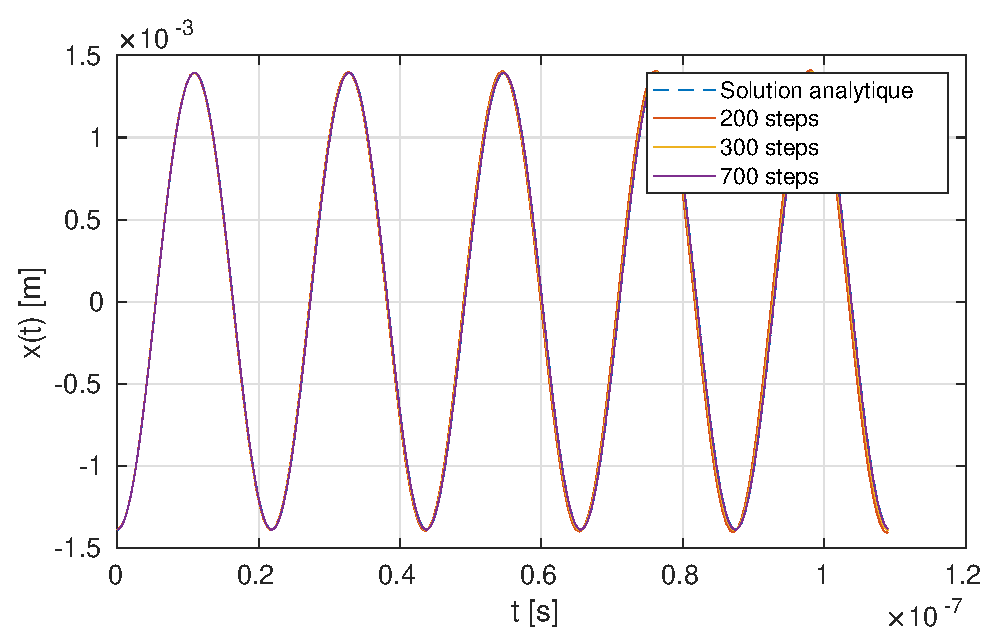
\includegraphics[scale=0.68,angle=0]{etudeSchema/etudeStabilitePosRungeKutta2}}
\caption{ \label{etudeStabilitePosRungeKutta2}\em
 Position sur x en fonction du temps avec $E=0$ et $B=B_0$, réalisé avec la méthode RK2.
}
\end{figure}
\begin{figure}[H]
\centerline{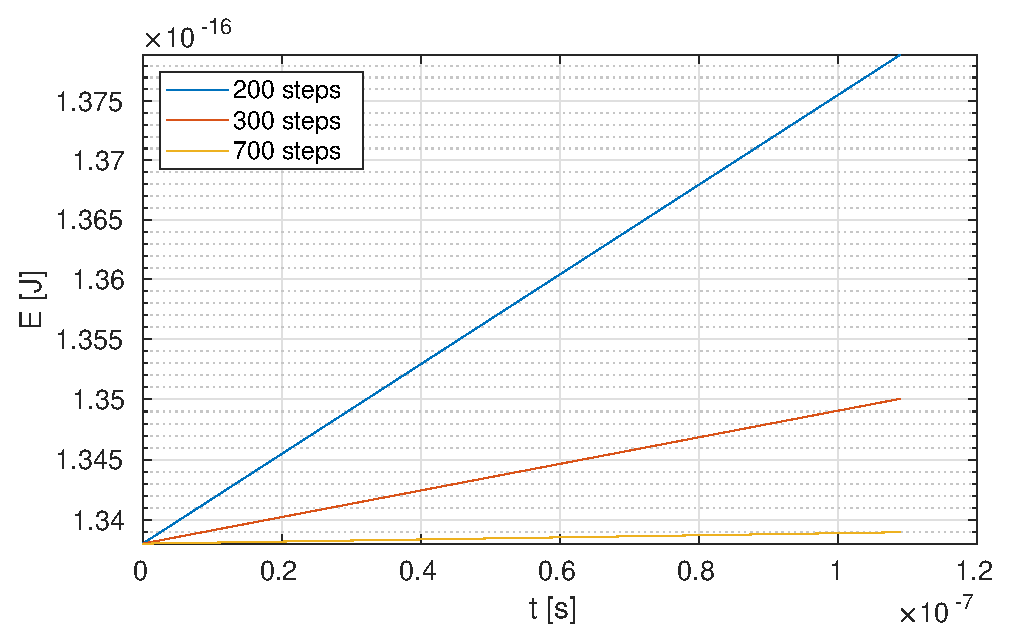
\includegraphics[scale=0.8,angle=0]{etudeSchema/etudeStabiliteEnergyRungeKutta2}}
\caption{ \label{etudeStabiliteEnergyRungeKutta2}\em
Énergie mécanique d'un proton en fonction du temps ($E=0$ et $B=B_0$), réalisé avec la méthode de RK2.
}
\end{figure}
\begin{figure}[H]
\centerline{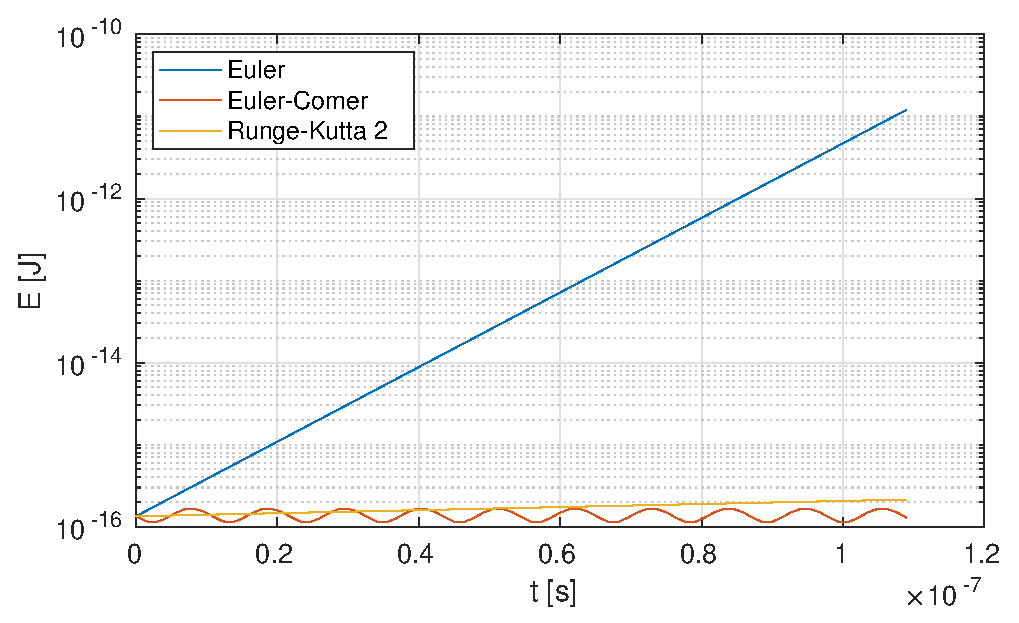
\includegraphics[scale=0.9,angle=0]{etudeSchema/etudeStabiliteCompEnergy}}
\caption{ \label{etudeStabiliteCompEnergy}\em
Comparaison des trois schémas pour $E=0$, $B=B_0$ et $N_{steps}=80$. L'énergie est conservée en moyenne pour Euler-Cromer contrairement aux deux autres.
}
\end{figure}


%%%%%%%%%%%%%%%%%%%%%%%%%%%%%%%%%%%%%%%%%%%%%%%%%%%%%%%%%%%%%%%%%%%%%%%%%%%%%%%%%%%%%%%%%%%%%%%%%%%%%%%%
\newpage
\subsection{Application 1 : dérive E $\times$ B}
Dans cette section, on considère la particule dans un champ magnétique et un champ électrique uniforme, de valeur $B=3 \rm T$ et $E=6\times10^4 \rm V/m$. On prendra les mêmes paramètres que pour les simulations précédentes concernant la vitesse et $t_{fin}$, c'est-à-dire $v_{x_0}=0$, $v_{y_0}=4\times 10^{5} \rm  m/s$ et $t_{fin}=1.09 \times 10^{-7} \rm s$. Les simulations sont faites uniquement avec le schéma de Runge-Kutta 2.

\subsubsection{Étude de convergence}
 Pour étudier la convergence, on effectue plusieurs simulations en augmentant $N_{steps}$ (le nombre de pas de temps). La position finale (à la fin de chaque simulation) en $x$ et $y$ est repésentée en fonction de $\Delta t$ sur la Fig.\ref{etudeConv1_1}. La position finale semble converger vers une valeur finie, tant en $x$ que en $y$.
 On peut confirmer l'ordre de convergence en représentant cette fois la position finale en fonction de $(\Delta t)^2$ (Fig.\ref{etudeConv1_2}). Nous obtenons une droite, confirmant que l'ordre de convergence est bien de 2.
\begin{figure}[H]
\centerline{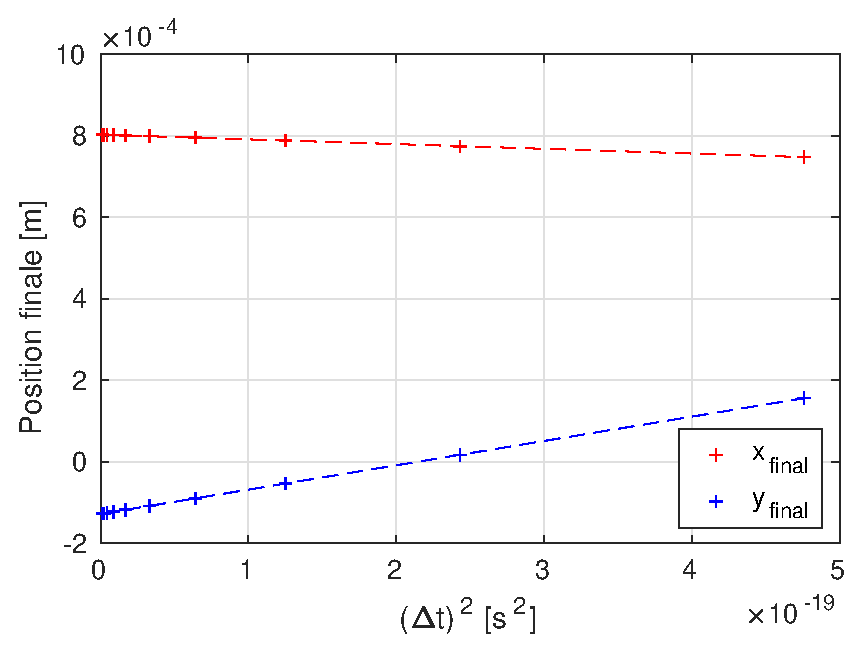
\includegraphics[width=0.95\linewidth,angle=0]{application1/etudeConv1_1}}
\caption{ \label{etudeConv1_1}\em
 Simulation avec la méthode RK2 d'un proton dans des champs magnétique et électriques uniformes. Position finale en fonction du pas de temps $\Delta t$. On peut constater que $x_{final}$ et $y_{final}$ convergent vers des valeurs finies.
}
\end{figure}

\begin{figure}[H]
\centerline{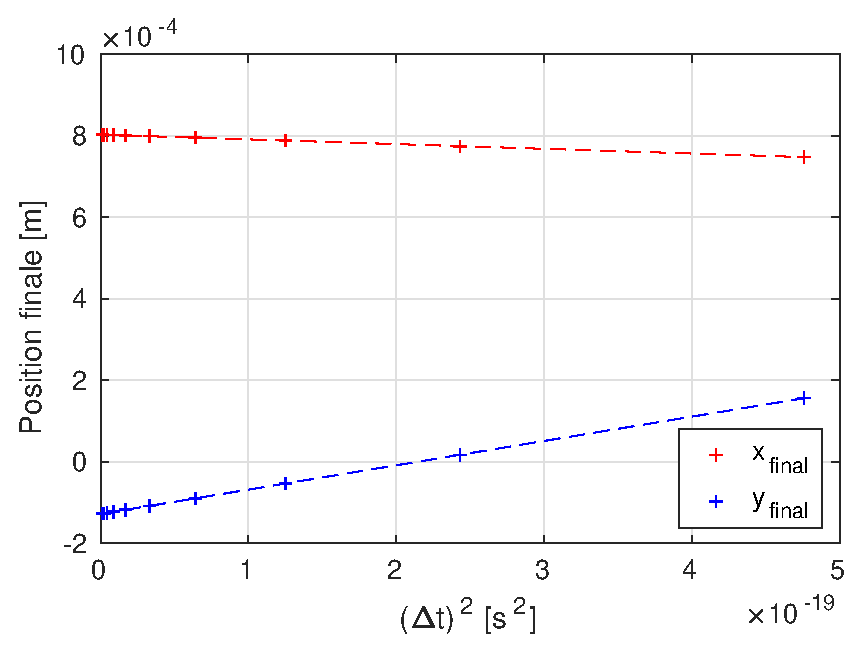
\includegraphics[width=0.78\linewidth,angle=0]{application1/etudeConv1_2}}
\caption{ \label{etudeConv1_2}\em
 Simulations d'un proton dans des champs magnétique et électrique uniformes avec la méthode RK2. En représentant la position finale en fonction de $(\Delta t)^2$, les points s'alignent, confirmant ainsi que l'ordre de convergence de la méthode RK2 est 2.
}
\end{figure}

\subsubsection{Énergie et trajectoires}
On étudie également l'évolution de l'énergie mécanique pour vérifier sa constance. On peut constater sur la Fig.\ref{RK2Energy1} que l'énergie n'est pas tout a fait conservée, illustrant à nouveau l'instabilité du schéma RK2.
\begin{figure}[H]
\centerline{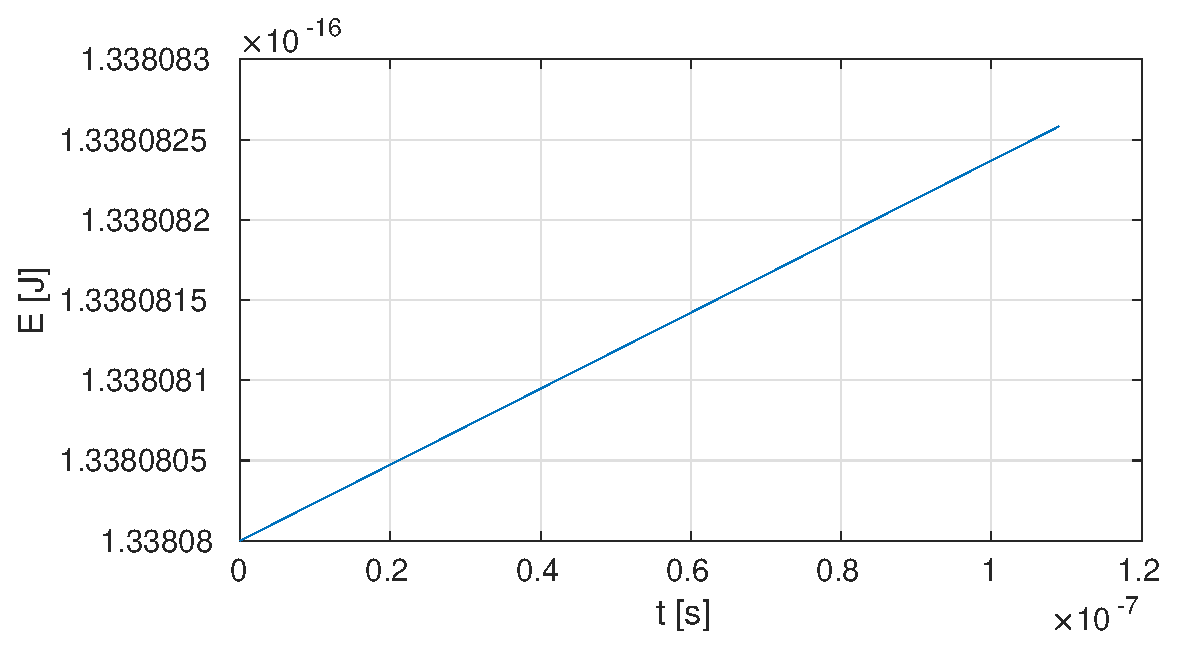
\includegraphics[width=0.8\linewidth,angle=0]{application1/RK2Energy1}}
\caption{ \label{RK2Energy1}\em
 Simulation avec la méthode RK2 d'un proton dans des champs magnétique et électrique uniformes avec $N_{steps}=500$. Le schéma de Runge-Kutta est très bon, mais on peut remarquer que l'énergie augmente très légèrement alors qu'elle devrait être conservée. Cette méthode n'est donc pas conservative.
}
\end{figure}

\begin{figure}[H]
\centerline{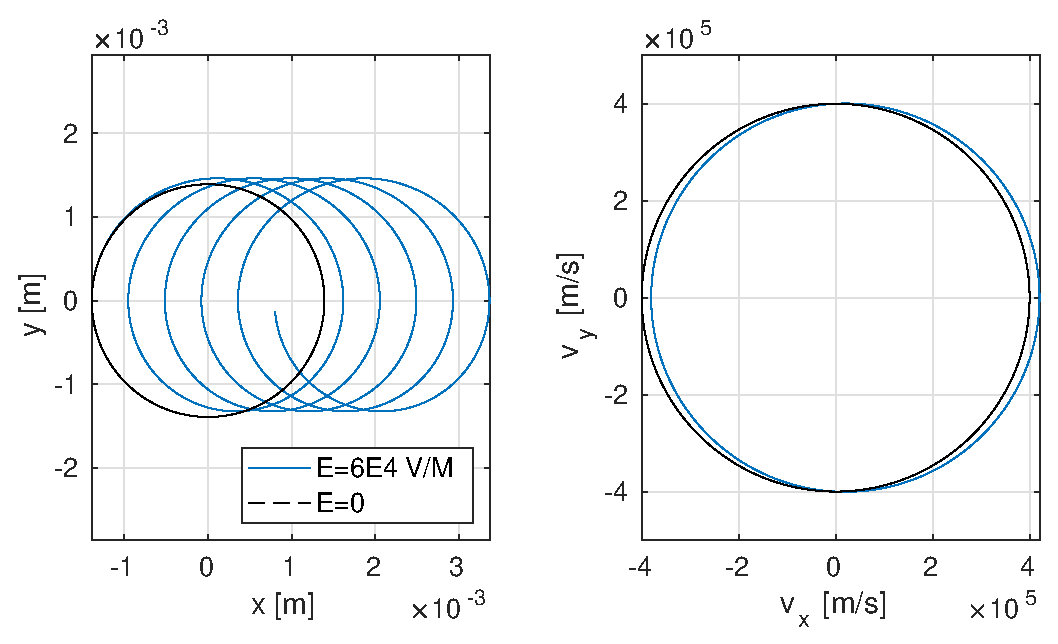
\includegraphics[width=0.85\linewidth,angle=0]{application1/RK2XY1}}
\caption{ \label{RK2XY1}\em
 Trajectoires d'un proton dans des champs électrique et magnétique uniformes dans un référentiel fixe (à gauche) et vitesse de la particule (à droite). Simulations réalisées avec la méthode RK2.
}
\end{figure}
La particule effectue un mouvement de type helicoïdal dans un référentiel fixe (Fig.\ref{RK2XY1}). C'est une superpsition d'un mouvement circulaire uniforme (MCU) et d'un mouvement de translation à vitesse constante (MRU). La trajectoire dans l'espace $(v_x,v_y)$ est quasiment la même que sans champ électrique, elle est juste légèrement décalée selon l'axe $v_x$.

Si on représente la trajectoire du proton dans un référentiel en translation uniforme $v_E=\norme{\textbf{E} \times \textbf{B}}/B^2$, on obtient la même trajectoire que dans le cas sans champ électrique (Fig.\ref{RK2XYvE1}). On peut en déduire que la vitesse de dérive du proton est égal à $v_E$.
\begin{figure}[H]
\centerline{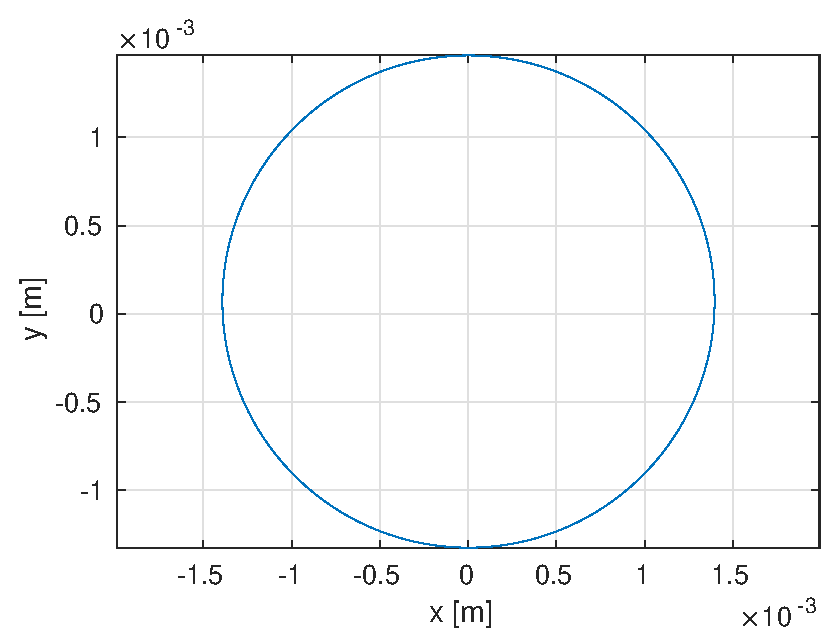
\includegraphics[width=0.55\linewidth,angle=0]{application1/RK2XYvE1}}
\caption{ \label{RK2XYvE1}\em
 Trajectoire d'un proton, en présence de champs magnétique et élctrique uniformes, représentée dans un référentiel en translation uniforme $v_E=\norme{\textbf{E} \times \textbf{B}}/B^2$. Simulations réalisées avec RK2.
}
\end{figure}

%%%%%%%%%%%%%%%%%%%%%%%%%%%%%%%%%%%%%%%%%%%%%%%%%%%%%%%%%%%%%%%%%%%%%%%%%%%%%%%%%%%%%%%%%%%%%%%%%%%%%%%%
\newpage
\subsection{Application 2 : dérive $\nabla B$}

On considère maintenant un champ d'intensité variable $\textbf{B}=B(x) \hat{z}$, avec $B(x)=(1+ \kappa x) B_0$, $\kappa = 100 \rm m^{-1}$, $B_0=3 \rm T$, $E=0$, $v_{x_0} = 0$, $v_{y_0}=4 \times 10^5 \rm m/s$ et $t_{fin}=1.09 \times 10^{-7} \rm s$. On réalise des simulations avec la méthode de Runge-Kutta 2.

On vérifie dans un premier temps que les solutions numériques convergent dans ce nouveau cas de figure. Comme la Fig.\ref{etudeConv2} le montre, il y a convergence et elle est d'ordre 2.

\begin{figure}[H]
\centerline{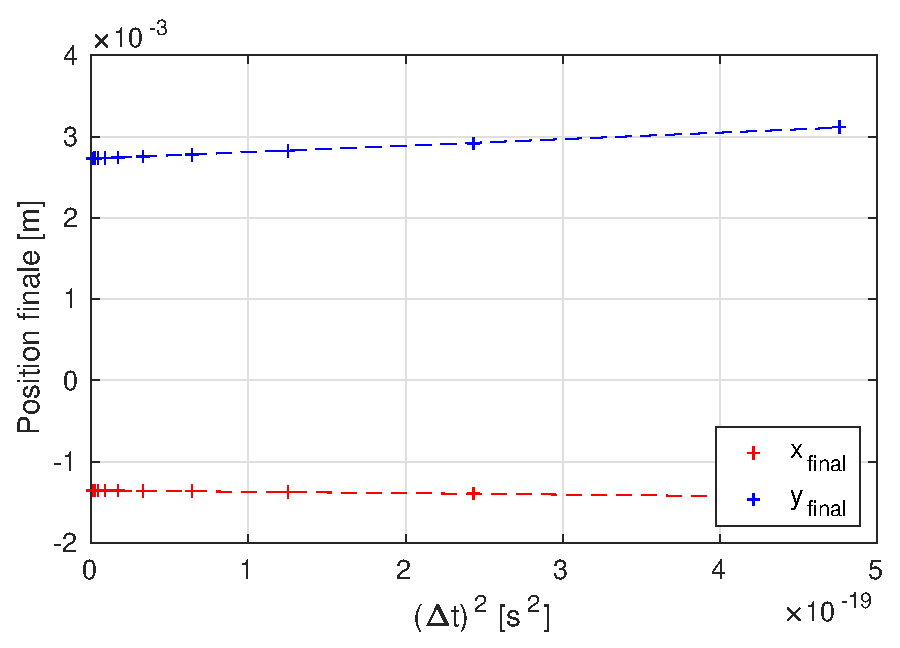
\includegraphics[width=0.9\linewidth,angle=0]{application2/etudeConv2}}
\caption{ \label{etudeConv2}\em
 Convergence quadratique de la méthode de Runge-Kutta 2 pour un proton dans un champ magnétique variable $\textbf{B}=B(x) \hat{z}$.
}
\end{figure}

On réalise maintenant une simulation pour un proton ($q=e$) avec $x_0= -1.39 \times 10^{-3} \rm m$, $y_0=0$ et une autre pour un antiproton ($q=-e$) avec $x_0= 1.39 \times 10^{-3} \rm m$, $y_0=0$. Les résultats de ces simulations sont présentés sur la Fig.\ref{comparaison2}. Les deux particules dérivent selon l'axe $y$, en plus de leur mouvement circulaire uniforme. On peut remarquer que leurs trajectoires sont symétriques dans le plan $(x,y)$, cependant les deux particules parcourent la même trajectoire dans l'espace $(v_x,v_y)$.

On se propose maintenant d'étudier la quantité $\mu = mv^2/2B$. Celle dernière oscille et est exactement l'inverse pour le proton et l'antiproton. Cependant elle est conservée en moyenne avec la même valeur moyenne pour les deux particules.

\begin{figure}[H]
\centerline{
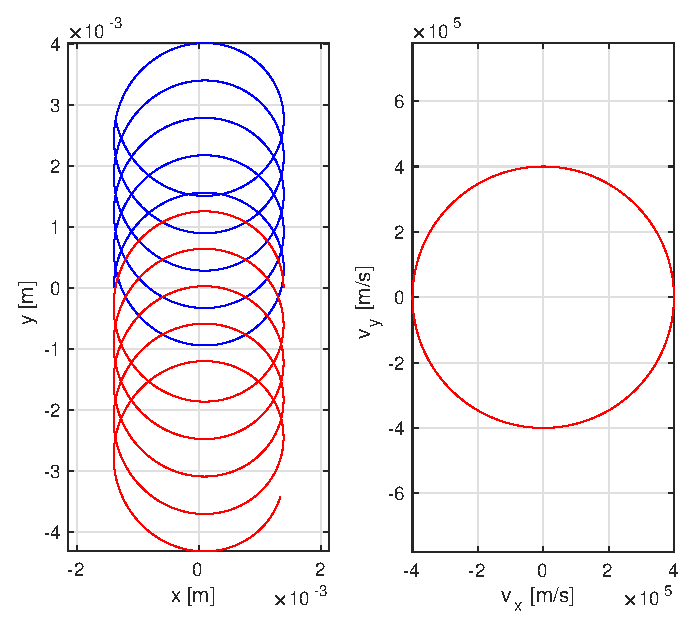
\includegraphics[width=0.533\linewidth,angle=0]{application2/comparaisonTrajectoire2}
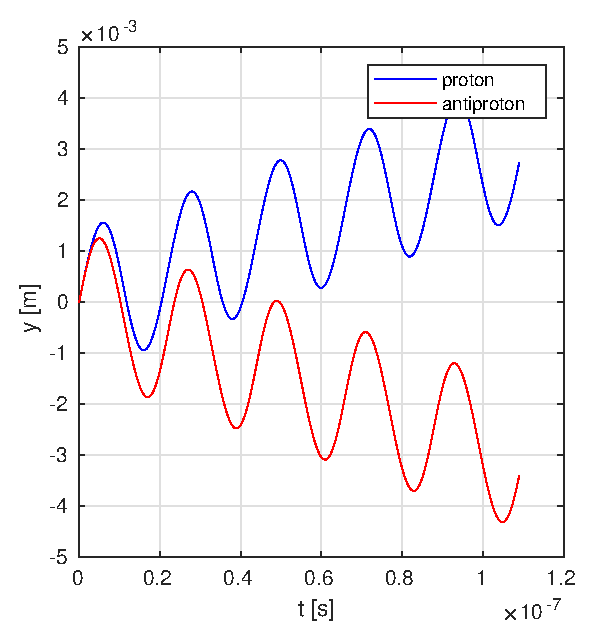
\includegraphics[width=0.45\linewidth,angle=0]{application2/comparaisonY2}}
\caption{ \label{comparaison2}\em
 Un proton (bleu) et un antiproton (rouge) dans un champ magnétique variable $\textbf{B}=B(x) \hat{z}$, simulé par la méthode de Runge-Kutta 2 avec $N_{steps}=5000$. Leurs positions en $\rm y$ présentent la même oscillation mais avec une vitesse de dérive opposée. 
}
\end{figure}

\begin{figure}[H]
\centerline{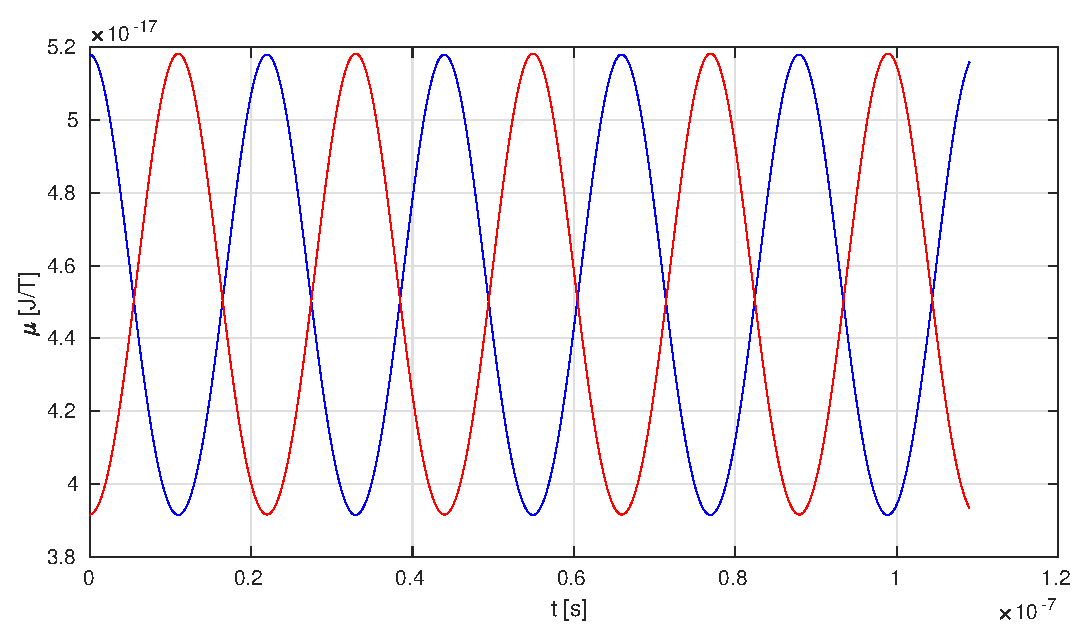
\includegraphics[width=0.9\linewidth,angle=0]{application2/comparaisonMu2}}
\caption{ \label{comparaisonMu2}\em
 La grandeur $\mu=mv^2/2B$ en fonction du temps pour un proton (bleu) et un antiproton (rouge) dans un champ magnétique variable $\textbf{B}=B(x) \hat{z}$, simulé par la méthode de Runge-Kutta 2 avec $N_{steps}=5000$.
}
\end{figure}

%%%%%%%%%%%%%%%%%%%%%%%%%%%%%%%%%%%%%%%%%%%%%%%%%%%%%%%%%%%%%%%%%%%%%%%%%%%%%%%%%%%%%%%%%%%%%%%%%%%%%%%%
\newpage
\section{Conclusion}
En conclusion, nous avons pu dans premier temps illustrer les propriétés de convergence, de stabilité et de conservation d'énergie pour les quatre méthodes numériques présentées, en connaissant la solution analytique, dans le cas d'un champ magnétique constant. Les ordres de convergence théoriques ont pu être confirmé et illustré par les essais numériques, tout comme la stabilité des ces schémas.
De plus, nous avons pu étudier le comportement de la méthode Runge-Kutta 2 dans deux cas d'applications où l'on ne connaît pas la solution analytique, ce qui illustre l'utilité des méthodes numériques.


%%%%%%%%%%%%%%%%%%%%%%%%%%%%%%%%%%%%%%%%%%%%%%%%%%%%%%%%%%%%%%%%%%%%%%%%%%%%%%%%%%%%%%%%%%%%%%%%%%%%%%%%
\begin{thebibliography}{99}
\bibitem{donneeEX2} 
Données de l'exercice 2. Laurent Villard, EPFL, 2018.
\bibitem{notesDeCours}
Physique numérique I/II, notes de cours. Laurent Villard, EPFL, 2018.
\bibitem{stubbe}
Analyse II, note de cours, pp.120-121. Joachim Stubbe, EPFL, 2018.
 \end{thebibliography}
\end{document}
